\section{Introduction}
\label{sec:intro}
In recent years, Large Language Models (LLMs), with their strong reasoning and generation capabilities, have been increasingly deployed in safety-critical domains such as autonomous driving
\cite{sima2024drivelm,tian2024drivevlm}, remote sensing analysis\cite{wang2025disasterm3}, medical diagnosis\cite{alsabbagh2025minimedgpt}, and industrial fault diagnosis \cite{chen2025faultgpt}. These models typically rely on large-scale GPUs or other AI accelerators, whose execution is susceptible to transient hardware faults induced by cosmic rays, voltage fluctuations, and device aging\cite{wang2023understanding,he2023understanding}. Such faults can silently alter computational results without triggering any system exception, forming Silent Data Corruption (SDC). Enterprises such as Meta and Google have reported the reliability challenges posed by SDC in large-scale GPU cluster operations \cite{grattafiori2024llama,vallin2025silent}. To address this, the Open Compute Project (OCP) established the Server Component Resilience Workstream, uniting Meta, Google, NVIDIA, and other companies to study SDC. Its whitepaper on SDC in AI explicitly points out that, in large-scale inference, SDC pollutes massive inference results and disrupts downstream task decisions, and that inference-side SDC further compromises data integrity and degrades model effectiveness \cite{ocp2025sdc}. SDC therefore remains a serious safety hazard in model inference scenarios.

To investigate the impact of SDC on LLM outputs, we conduct extensive fault injection experiments, with results shown in Figure~\ref{fig:1}. Figures~\ref{fig:1}a and b show cases where the SDC does not change the semantics of the output and thus does not alter the model's decision; in contrast, Figures~\ref{fig:1}c and d show faulty outputs with severe semantic deviations that substantially affect the model's decision. We define SDCs that induce such significant semantic deviations as \textbf{Significant SDCs}; in safety-critical scenarios such as autonomous driving, this class of errors may cause severe consequences and is therefore the detection target of this work.

\begin{figure}[!ht]
\centering
    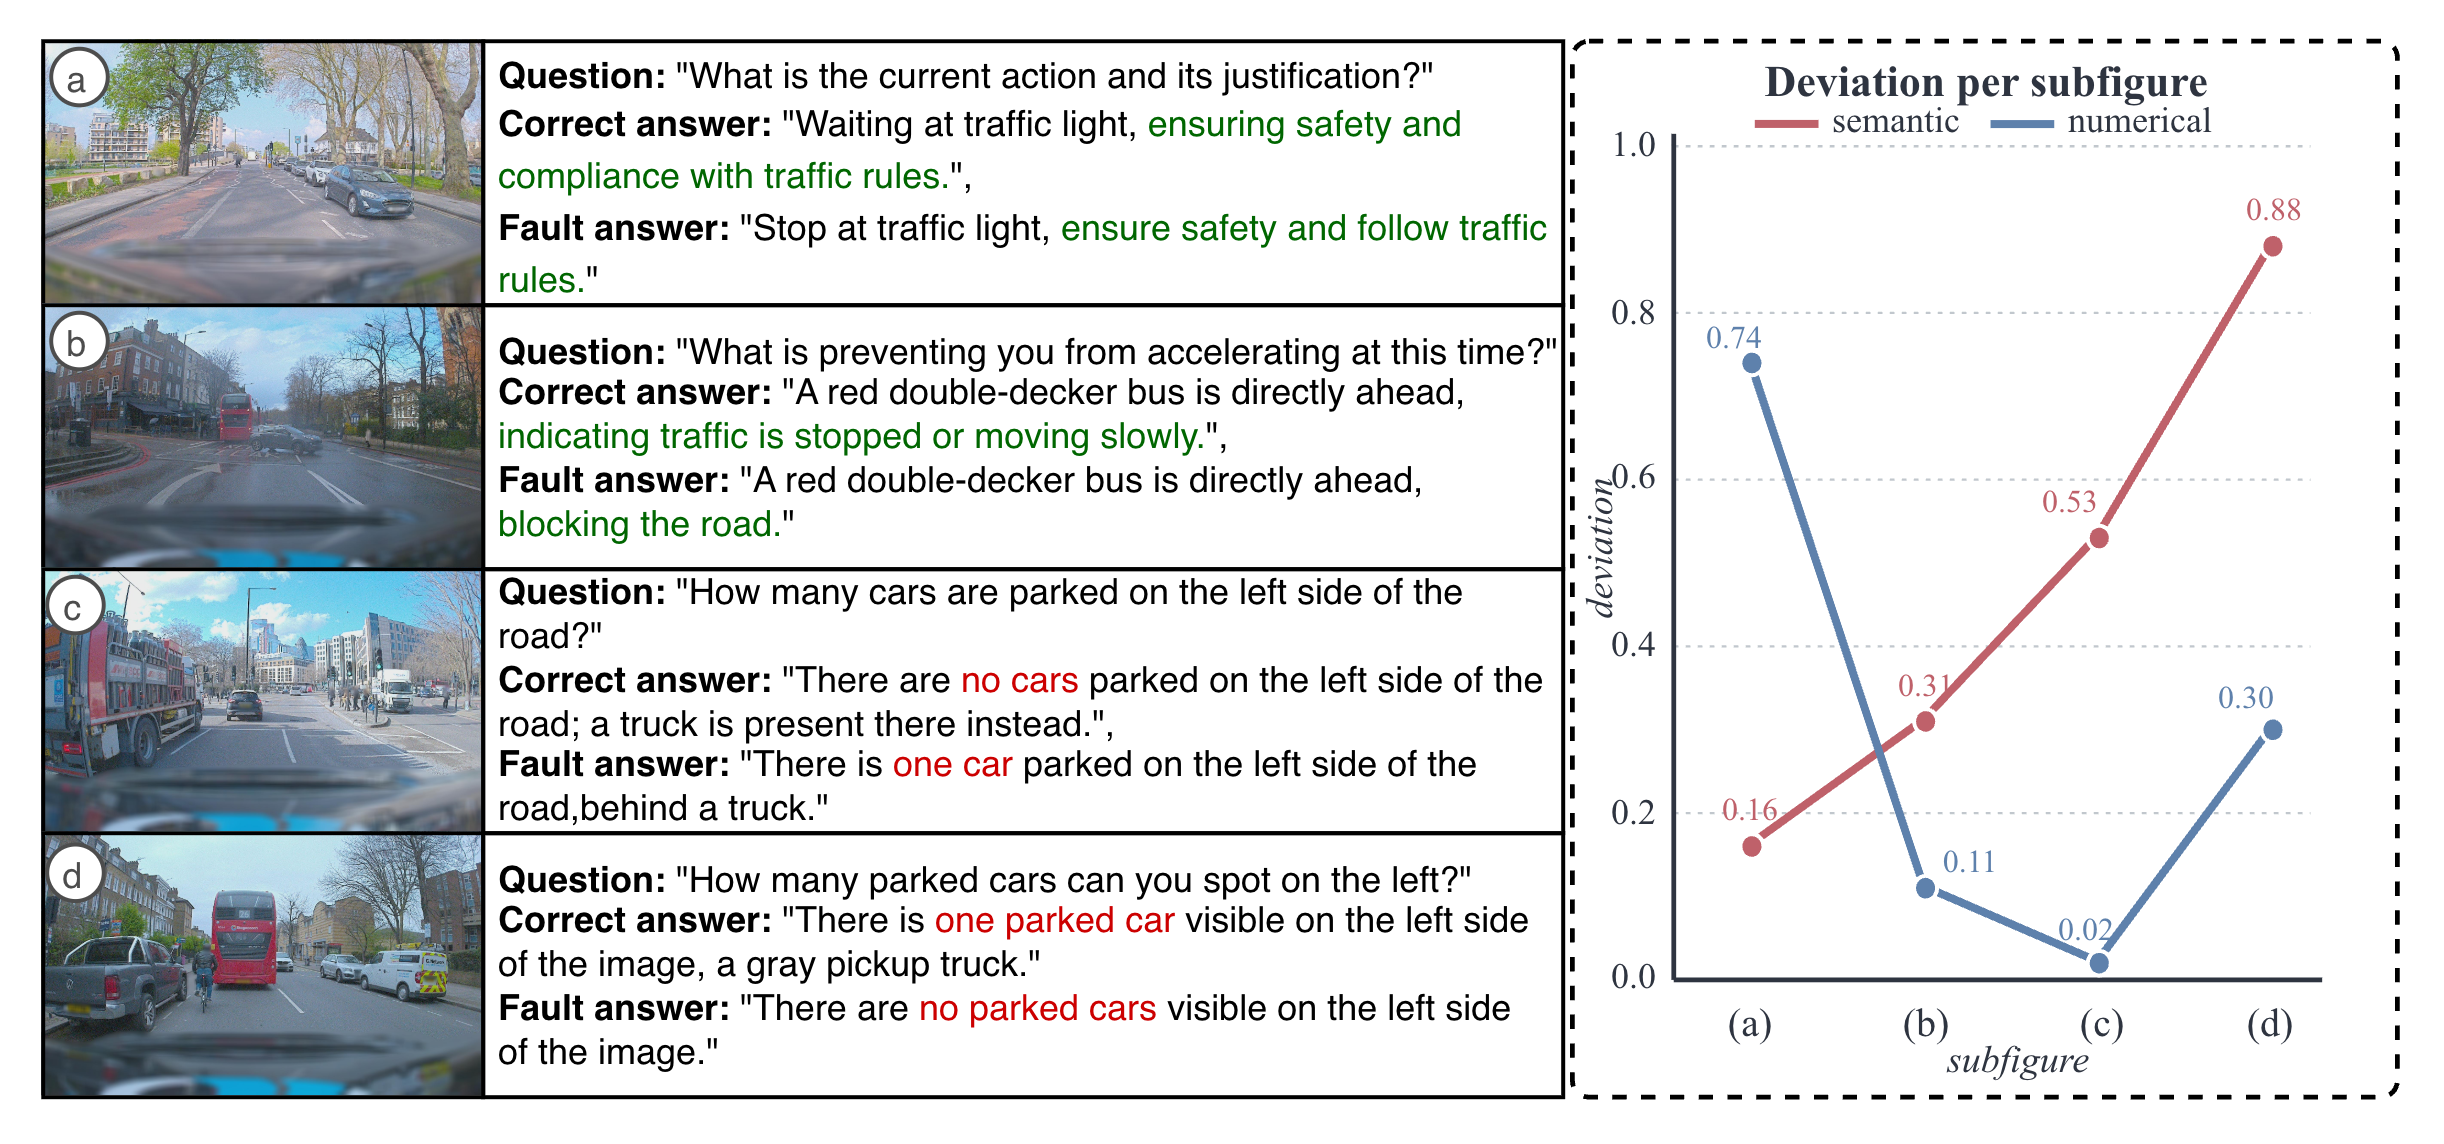
\includegraphics[width=1.0\linewidth]{Figures/figure1_examples_of_SDC_outputs.png}
    \caption{Examples of SDC outputs with different numerical and semantic deviations. The line chart (right) plots the two deviation types per subfigure, showing they do not correspond.}
    \label{fig:1}
\end{figure}

Existing soft error detection methods, such as Ranger and Dr.DNA, typically assess fault impact based on the activation range or numerical distribution. However, as the line chart in Figure~\ref{fig:1} illustrates, there is no one-to-one correspondence between the numerical deviation and the semantic deviation of the output in LLMs: a large numerical perturbation may be absorbed by subsequent computation, while a small one may propagate through the network and alter key generated content. Methods with fixed numerical thresholds therefore tend to suffer from both missed Significant SDCs and false alarms on non-critical faults. An effective detector must further characterize how faults affect the semantic representations inside the model.

We propose \textbf{SIEVE}, a lightweight, semantics-aware soft error detection framework for LLMs. SIEVE monitors selected adjacent decoder layers during inference, projects their intermediate representations into a low-dimensional space, and uses a Nominal Inter-Layer Predictor trained on clean execution traces to model the nominal inter-layer mapping. At runtime, the deviation of the actual representations from this mapping is aggregated into a layer-wise \textbf{Discrepancy Profile}; after further aggregation over multiple decoding steps, an independently calibrated lightweight classifier judges whether the current execution suffers a Significant SDC.

We systematically evaluate SIEVE on three representative LLMs and three VQA datasets. Under an evaluation protocol with semantically isolated splits and frozen thresholds (\S\ref{sec:experiments}), SIEVE achieves a macro-average F1 of 93.78\% and a non-Significant-SDC false positive rate of 0.107\% on the Test set of the nine tasks, with an end-to-end overhead of about 6.65\%, substantially outperforming the Ranger and Dr.DNA baselines under identical configurations.

Our main contributions are summarized as follows:
\begin{itemize}
  \item We formulate the Significant SDC problem for LLM inference, and reveal through systematic fault injection the inconsistency between the magnitude of numerical anomalies and the final semantic damage, thereby arguing the inherent limitations of the numerical-threshold detection paradigm.
  \item We propose SIEVE, a lightweight online Significant SDC detection framework. SIEVE learns the nominal transformation of representations between adjacent layers from clean traces, and constructs a Discrepancy Profile from the deviation between predicted and actual representations as the detection signal for Significant SDCs, which a lightweight classifier then judges.
  \item We conduct a unified evaluation on three LLMs and three VQA datasets. Under the best configuration, SIEVE achieves a macro-average F1 of 93.78\%, a recall of 91.49\%, and an FPR of 0.107\% on the Test set, improving over same-configuration baselines by up to 11.38 percentage points.
\end{itemize}

